\documentclass[11pt,a4paper]{article}

\usepackage{filecontents}
\begin{filecontents*}{\jobname.bib}
  @misc{zenoh-tls,
    author = {{Eclipse Zenoh}},
    title = {{TLS authentication}},
    year = {2024},
    howpublished = {\url{https://zenoh.io/docs/manual/tls/}},
    note = {Accessed 22 April 2026}
  }
  @misc{zenoh-config,
    author = {{Eclipse Zenoh}},
    title = {{Zenoh Default Configuration (DEFAULT\_CONFIG.json5)}},
    year = {2024},
    howpublished =
    {\url{https://github.com/eclipse-zenoh/zenoh/blob/main/DEFAULT_CONFIG.json5}},
    note = {Accessed 22 April 2026}
  }
  @misc{zenoh-acl,
    author = {{Eclipse Zenoh}},
    title = {{Access Control}},
    year = {2024},
    howpublished = {\url{https://zenoh.io/docs/manual/access-control/}},
    note = {Accessed 22 April 2026}
  }
  @misc{zenoh-acl-rfc,
    author = {{Eclipse Zenoh}},
    title = {{Access Control Rules RFC}},
    year = {2024},
    howpublished =
    {\url{https://github.com/eclipse-zenoh/roadmap/blob/main/rfcs/ALL/Access\%20Control\%20Rules.md}},
    note = {Accessed 22 April 2026}
  }
  @misc{zenoh-deployment,
    author = {{Eclipse Zenoh}},
    title = {{Deployment}},
    year = {2024},
    howpublished = {\url{https://zenoh.io/docs/getting-started/deployment/}},
    note = {Accessed 22 April 2026}
  }
  @misc{zenoh-firesong,
    author = {{Eclipse Zenoh}},
    title = {{Zenoh 1.0.0 ``Firesong'' is ready to rock!}},
    howpublished = {\url{https://zenoh.io/blog/2024-10-21-zenoh-firesong/}},
    year = {2024},
    note = {Accessed 22 April 2026}
  }
  @misc{rfc6762,
    author = {S. Cheshire and M. Krochmal},
    title = {{Multicast DNS}},
    howpublished = {RFC 6762, IETF},
    year = {2013},
    note = {\url{https://www.rfc-editor.org/rfc/rfc6762}}
  }
  @misc{rfc4795,
    author = {B. Aboba and D. Thaler and L. Esibov},
    title = {{Link-local Multicast Name Resolution (LLMNR)}},
    howpublished = {RFC 4795, IETF (Informational)},
    year = {2007},
    note = {\url{https://datatracker.ietf.org/doc/html/rfc4795}}
  }
  @misc{ms-mdns,
    author = {{Microsoft}},
    title = {{Aligning on mDNS: ramping down NetBIOS name resolution
    and LLMNR}},
    howpublished = {Microsoft Networking Blog},
    year = {2022},
    note =
    {\url{https://techcommunity.microsoft.com/blog/networkingblog/aligning-on-mdns-ramping-down-netbios-name-resolution-and-llmnr/3290816}}
  }
  @misc{avahi,
    author = {{Avahi Project}},
    title = {{Avahi: mDNS/DNS-SD service discovery}},
    year = {2024},
    howpublished = {\url{https://avahi.org/}},
    note = {Accessed 22 April 2026}
  }
  @misc{mdnssd,
    author = {Xianjun Jiao and contributors},
    title = {{mdns-sd: pure-Rust mDNS/DNS-SD client and responder}},
    year = {2024},
    howpublished = {\url{https://crates.io/crates/mdns-sd}},
    note = {Accessed 9 June 2026}
  }
  @misc{stepca,
    author = {{Smallstep}},
    title = {{step-ca: an online certificate authority}},
    year = {2024},
    howpublished = {\url{https://smallstep.com/docs/step-ca/}},
    note = {Accessed 9 June 2026}
  }
  @misc{keycloak,
    author = {{Keycloak Project}},
    title = {{Keycloak: Open-Source Identity and Access Management}},
    year = {2024},
    howpublished = {\url{https://www.keycloak.org/}},
    note = {Accessed 9 June 2026}
  }
  @misc{rcgen,
    author = {est31 and contributors},
    title = {{rcgen: Rust X.509 certificate generation}},
    year = {2024},
    howpublished = {\url{https://crates.io/crates/rcgen}},
    note = {Accessed 9 June 2026}
  }
  @misc{rfc8446,
    author = {E. Rescorla},
    title = {{The Transport Layer Security (TLS) Protocol Version 1.3}},
    howpublished = {RFC 8446, IETF},
    year = {2018},
    note = {\url{https://www.rfc-editor.org/rfc/rfc8446}}
  }
  @misc{rfc5280,
    author = {D. Cooper and S. Santesson and S. Farrell and S. Boeyen
    and R. Housley and W. Polk},
    title = {{Internet X.509 Public Key Infrastructure Certificate
    and Certificate Revocation List (CRL) Profile}},
    howpublished = {RFC 5280, IETF},
    year = {2008},
    note = {\url{https://www.rfc-editor.org/rfc/rfc5280}}
  }
\end{filecontents*}

\usepackage[margin=2.5cm]{geometry}
\usepackage{fontspec}
\setmainfont{Latin Modern Roman}
\setsansfont{Latin Modern Sans}
\setmonofont{Hack}[Scale=0.85]
\usepackage{amssymb}
\usepackage{amsmath}
\usepackage{graphicx}
\usepackage[dvipsnames,table]{xcolor}
\usepackage{tikz}
\usetikzlibrary{positioning,arrows.meta,fit,backgrounds,shapes.geometric,calc,decorations.pathmorphing}
\usepackage{listings}
\usepackage{enumitem}
\usepackage{hyperref}
\usepackage{fancyhdr}
\usepackage{titlesec}
\usepackage{parskip}
\usepackage{float}
\usepackage{booktabs}
\usepackage{array}
\usepackage{adjustbox}
\usepackage[numbers,square,sort&compress]{natbib}
\usepackage[most]{tcolorbox}

% Colors
\definecolor{router}{HTML}{E74C3C}
\definecolor{peer}{HTML}{3498DB}
\definecolor{client}{HTML}{2ECC71}
\definecolor{admitted}{HTML}{2ECC71}
\definecolor{denied}{HTML}{E74C3C}
\definecolor{nocert}{HTML}{95A5A6}
\definecolor{central}{HTML}{9B59B6}
\definecolor{session}{HTML}{3498DB}
\definecolor{discover}{HTML}{F39C12}
\definecolor{tls}{HTML}{2ECC71}
\definecolor{pubkey}{HTML}{2ECC71}
\definecolor{privkey}{HTML}{E74C3C}
\definecolor{msgcol}{HTML}{3498DB}
\definecolor{cipher}{HTML}{9B59B6}
\definecolor{ca}{HTML}{F39C12}
\definecolor{cert}{HTML}{3498DB}
\definecolor{domaincol}{HTML}{2ECC71}
\definecolor{agent}{HTML}{3498DB}
\definecolor{machine}{HTML}{ECF0F1}
\definecolor{avahi}{HTML}{9B59B6}
\definecolor{transport}{HTML}{95A5A6}
\definecolor{session1}{HTML}{3498DB}
\definecolor{session2}{HTML}{F39C12}
\definecolor{othersession}{HTML}{F39C12}
\definecolor{codebg}{HTML}{F8F8F8}
\definecolor{codeframe}{HTML}{DDDDDD}
\definecolor{nixblue}{HTML}{5277C3}
\definecolor{soft}{HTML}{F4F6F8}

% Abstract box styling
\newtcolorbox{abstractbox}[1][]{
  enhanced, colback=soft, colframe=nixblue,
  boxrule=0.6pt, arc=2pt, left=10pt, right=10pt, top=8pt, bottom=8pt,
  title=\textbf{Abstract}, coltitle=white, colbacktitle=nixblue,
  fonttitle=\sffamily\bfseries, #1
}

% Listings style
\lstset{
  basicstyle=\ttfamily\small,
  backgroundcolor=\color{codebg},
  frame=single,
  rulecolor=\color{codeframe},
  breaklines=true,
  breakatwhitespace=true,
  tabsize=2,
  showstringspaces=false,
  keywordstyle=\color{blue},
  stringstyle=\color{red!70!black},
  commentstyle=\color{green!50!black},
}

% Header/footer
\pagestyle{fancy}
\fancyhf{}
\fancyhead[L]{\small\textit{Zenoh security architecture for DVerse}}
\fancyhead[R]{\small\textit{DVerse Platform}}
\fancyfoot[C]{\thepage}
\renewcommand{\headrulewidth}{0.4pt}

% Hyperlinks
\hypersetup{
  colorlinks=true,
  linkcolor=blue!60!black,
  urlcolor=blue!60!black,
  citecolor=blue!60!black,
}

\title{%
  \vspace{-1cm}
  {\LARGE\bfseries Zenoh Security Architecture for AI Agent
  Communication in the DVerse Platform}
}
\author{Yordan Mitev}
\date{\today}

\begin{document}

\maketitle
\thispagestyle{fancy}

% ==============================================================
% Abstract in a box
% ==============================================================
\begin{abstractbox}
  This document evaluates Zenoh as the messaging backbone for the
  DVerse platform, a decentralized system for AI agent communication.
  It reports the findings from two phases of work. The first phase
  validated the basic pub/sub mechanics of Zenoh using a ping-pong
  demo in Rust. The second phase focused on security and local
  discovery. It covers mutual TLS authentication, certificate
  management, and local node discovery using mDNS (V3 moved this
  from the system-level Avahi daemon to the in-process
  \texttt{mdns-sd} Rust crate). The
  document also proposes a platform architecture in which each
  machine runs a central Zenoh router with local agents, and routers
  on different machines form an authenticated mesh. The scope of this
  document is limited to the security and communication aspects of
  the architecture. How agents themselves are constructed is out of
  scope and will be covered in a separate document once that design
  is clearer. The third phase (V3) records the move away from static
  Zenoh ACLs as the only access control mechanism. Static ACLs cannot
  be reloaded at runtime: every change of the admitted set requires
  closing and reopening the Zenoh session, which interrupts the
  continuous availability the platform exists to provide. V3
  introduces a cryptographic admission handshake on top of mTLS, with
  per-session Megolm encryption of every payload and a wire relay that
  distributes per-process session keys to cross-machine agents.
  Certificate enrolment runs through a Keycloak~+ OIDC~+ Step-CA
  pipeline, and discovery moved from the system-level Avahi daemon
  to the in-process \texttt{mdns-sd} Rust crate. The
  remaining topic-level access control is retained as open work.
  The multi-session idea originally listed as a ``wacky'' future
  direction in V2 turned out to be exactly what the V3 admission +
  Megolm pivot delivers, so it has been rewritten in the past tense.
\end{abstractbox}

\vspace{1em}

\begin{table}[H]
  \centering
  \small
  \begin{tabular}{|l|l|p{7.5cm}|}
    \hline
    \rowcolor{gray!15}
    \textbf{Version} & \textbf{Date} & \textbf{Changes} \\
    \hline
    V1 & 10 March 2026 & Initial evaluation of Zenoh pub/sub
    with a ping-pong demo. \\
    \hline
    V2 & 22 April 2026 & Added TLS/mTLS, local discovery, and
    platform architecture. \\
    \hline
    V3 & 9 June 2026 & Recorded the pivot from static ACLs to
    admission + Megolm; documented the Keycloak/OIDC/Step-CA
    enrolment pipeline and the move from Avahi to the
    \texttt{mdns-sd} crate. \\
    \hline
  \end{tabular}
  \caption{Revision history.}
  \label{tab:history}
\end{table}

\newpage
\tableofcontents
\newpage
\listoffigures
\vspace{1em}
\listoftables
\vspace{1em}
\renewcommand{\lstlistlistingname}{List of Listings}
\lstlistoflistings
\newpage

% ==============================================================
\section{Introduction}
% ==============================================================

This document presents the evaluation of Zenoh as the messaging
backbone for the DVerse platform. The DVerse platform is a
decentralized system for AI agent communication. The goal is to let
multiple AI agents talk to each other over a transparent topology,
without a central broker or single point of control.

A decentralized architecture is essential for this platform. Agents
may be operated by different parties and run across different
networks. They need to form communication meshes without relying on a
coordinating server. Zenoh was chosen as a candidate because it
supports peer-to-peer and routed communication modes, low-latency
pub/sub messaging, and built-in TLS security~\citep{zenoh-tls,zenoh-deployment}.

This document is structured in two phases. The first phase (V1)
covers the initial evaluation of Zenoh's core pub/sub mechanics. The
second phase (V2) covers TLS security, local node discovery, and the
resulting platform architecture.

\subsection{Scope}

The scope of this document is the security and communication layer of
the DVerse platform. It describes how Zenoh nodes are authenticated,
how they discover each other on a local network, and how sessions of
authenticated routers are formed. It does not describe how the agents
themselves are built, what their internal logic looks like, or how
they interact with application-level APIs. That part of the design is
still evolving and will be addressed in a separate document once it has settled.

% ==============================================================
\section{Why Zenoh}
% ==============================================================

In a decentralized agent platform, agents need to discover and talk
to each other without depending on a central authority. Traditional
message brokers such as MQTT brokers, NATS servers, and RabbitMQ
introduce a central point of failure, a single point of control, and
an opaque routing layer. These properties conflict with a decentralized design.

Zenoh was selected for several reasons, each described below.

\subsection{Decentralized by Design}
Zenoh does not require a central broker. Agents can communicate
directly in peer-to-peer mode or through optional
routers~\citep{zenoh-deployment}. There is no single point of failure
or control. New agents can join the mesh without registering with a
central server.

\subsection{Transparent Topology}
Zenoh supports peer-to-peer, client-router, and fully meshed
configurations~\citep{zenoh-deployment}. The topology is visible and
configurable rather than hidden behind a broker abstraction.
Operators can see how agents are connected.

\subsection{Security}
Zenoh provides TLS and mutual TLS (mTLS) for encrypted, authenticated
communication between nodes~\citep{zenoh-tls}. This is essential when
agents may run across different hosts, networks, or trust boundaries.

\subsection{Simplicity}
The API surface is small. Declaring subscribers, publishing messages,
and loading configuration from files are all straightforward
operations~\citep{zenoh-config}.

\subsection{Performance}
Zenoh is designed for high-throughput, low-latency
scenarios~\citep{zenoh-firesong}. This matters as the number of
agents and the message volume grow.

% ==============================================================
\section{Zenoh Topologies}
% ==============================================================

Zenoh supports three communication
topologies~\citep{zenoh-deployment}. The choice of topology
determines how nodes discover each other, how messages are routed,
and what trade-offs exist between flexibility, performance, and
control. Each topology is described in its own subsection below.

\subsection{Peer-to-Peer}

Peer-to-peer mode lets nodes connect directly to each other without
any intermediary, as shown in Figure~\ref{fig:topology-p2p}. Every
node can publish and subscribe, and messages flow directly between
peers. This gives the lowest latency but requires every peer to know
about every other peer, which does not scale well.

\begin{figure}[H]
  \centering
  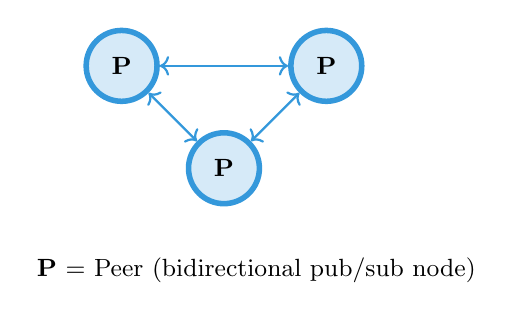
\begin{tikzpicture}[
      pr/.style={circle, draw=peer, fill=peer!20, line width=2pt,
      minimum size=0.9cm, font=\bfseries\small},
      link/.style={-{Stealth[length=3mm]}, thick, <->},
    ]
    \node[pr] (p1) at (-1.3, 1.3) {P};
    \node[pr] (p2) at (1.3, 1.3) {P};
    \node[pr] (p3) at (0, 0) {P};
    \draw[link, peer] (p1) -- (p2);
    \draw[link, peer] (p2) -- (p3);
    \draw[link, peer] (p1) -- (p3);

    % Legend
    \node[font=\small, anchor=west] at (-2.5, -1.3) {\textbf{P} =
    Peer (bidirectional pub/sub node)};
  \end{tikzpicture}
  \caption{Peer-to-peer topology. Every peer connects directly to
  every other peer.}
  \label{fig:topology-p2p}
\end{figure}

\subsection{Client-Router}

Client-router mode introduces a router that acts as a hub, as shown
in Figure~\ref{fig:topology-cr}. Clients connect to the router and
communicate through it. The router handles message routing and
forwarding. This is simpler to configure and scales better than
peer-to-peer, but the router must be available.

\begin{figure}[H]
  \centering
  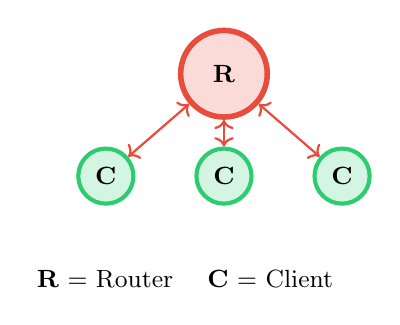
\begin{tikzpicture}[
      rtr/.style={circle, draw=router, fill=router!20, line
      width=2pt, minimum size=1.1cm, font=\bfseries\small},
      cl/.style={circle, draw=client, fill=client!20, line
      width=1.5pt, minimum size=0.7cm, font=\bfseries\small},
      link/.style={-{Stealth[length=3mm]}, thick, <->},
    ]
    \node[rtr] (r1) at (0, 1.3) {R};
    \node[cl] (c1) at (-1.5, 0) {C};
    \node[cl] (c2) at (0, 0) {C};
    \node[cl] (c3) at (1.5, 0) {C};
    \draw[link, router] (r1) -- (c1);
    \draw[link, router] (r1) -- (c2);
    \draw[link, router] (r1) -- (c3);

    % Legend
    \node[font=\small, anchor=west] at (-2.5, -1.3) {\textbf{R} =
    Router \quad \textbf{C} = Client};
  \end{tikzpicture}
  \caption{Client-router topology. Clients connect to a router that
  handles all message routing.}
  \label{fig:topology-cr}
\end{figure}

\subsection{Router Mesh}

Router mesh mode connects multiple routers, each with their own set
of clients, as shown in Figure~\ref{fig:topology-mesh}. Routers
forward messages between each other, creating a distributed routing
fabric. This combines the scalability of client-router mode with
redundancy. This is the topology chosen for the DVerse platform.

\begin{figure}[H]
  \centering
  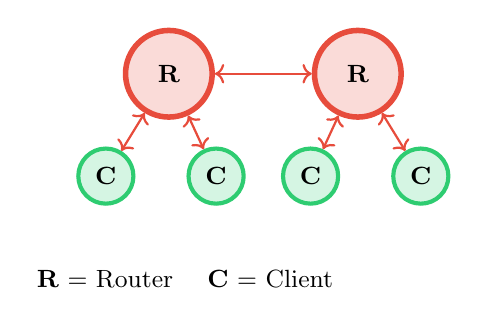
\begin{tikzpicture}[
      rtr/.style={circle, draw=router, fill=router!20, line
      width=2pt, minimum size=1.1cm, font=\bfseries\small},
      cl/.style={circle, draw=client, fill=client!20, line
      width=1.5pt, minimum size=0.7cm, font=\bfseries\small},
      link/.style={-{Stealth[length=3mm]}, thick, <->},
    ]
    \node[rtr] (r2) at (-1.2, 1.3) {R};
    \node[rtr] (r3) at (1.2, 1.3) {R};
    \draw[link, router] (r2) -- (r3);
    \node[cl] (c4) at (-2, 0) {C};
    \node[cl] (c5) at (-0.6, 0) {C};
    \node[cl] (c6) at (0.6, 0) {C};
    \node[cl] (c7) at (2, 0) {C};
    \draw[link, router] (r2) -- (c4);
    \draw[link, router] (r2) -- (c5);
    \draw[link, router] (r3) -- (c6);
    \draw[link, router] (r3) -- (c7);

    % Legend
    \node[font=\small, anchor=west] at (-3, -1.3) {\textbf{R} =
    Router \quad \textbf{C} = Client};
  \end{tikzpicture}
  \caption{Router mesh topology. Multiple routers connect to each
  other and each serves local clients.}
  \label{fig:topology-mesh}
\end{figure}

% ==============================================================
\section{V1 Findings: Core Pub/Sub}
% ==============================================================

\subsection{What Was Built}

A minimal ping-pong demo consisting of two Rust services was
implemented. The goal was to validate the developer experience and
the core pub/sub mechanics. The pong service subscribes to the
\texttt{ping} topic, logs received messages, and publishes a response
to the \texttt{pong} topic with its own identifier. The ping service
does the reverse.

\subsection{Results}

The evaluation confirmed that Zenoh's pub/sub model is easy to work
with in Rust. Setting up sessions, subscribing to topics, and
publishing messages required very little boilerplate. Configuration
management with file-based configs and fallback defaults worked as
expected~\citep{zenoh-config}.

The transparent, decentralized topology model is a good fit for the
agent platform. Agents can be deployed in various network
configurations without changing application code. Only the Zenoh
config needs to change. No central broker was required at any point
during the demo. The two services communicated directly, which
validated the decentralized approach.

% ==============================================================
\section{V2 Findings: TLS Security}
% ==============================================================

Security is important in a decentralized system because there is no
central authority gatekeeping access. The second phase of the
evaluation focused on implementing TLS and mutual TLS (mTLS) so that
all communication between Zenoh nodes is encrypted and mutually
authenticated~\citep{zenoh-tls,rfc8446}.

\subsection{Asymmetric Cryptography}

TLS is built on asymmetric (public-key) cryptography. In this scheme,
each party holds a pair of mathematically linked keys: a public key
that can be shared freely, and a private key that must be kept
secret. Data encrypted with the public key can only be decrypted with
the matching private key, and vice versa. Figure~\ref{fig:asymmetric}
shows this process.

\begin{figure}[H]
  \centering
  \begin{adjustbox}{max width=\textwidth}
    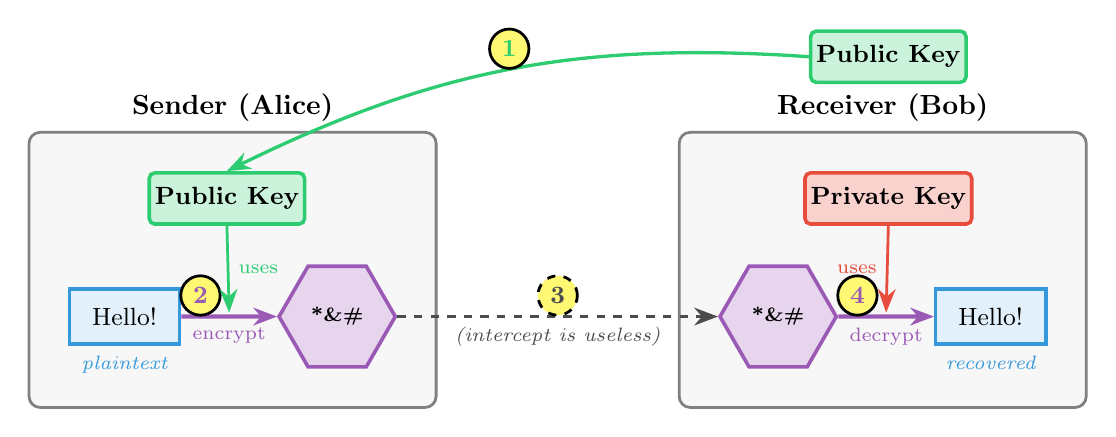
\begin{tikzpicture}[
        actorbox/.style={rectangle, rounded corners, draw=black!50,
        fill=black!3, line width=1pt, inner sep=14pt},
        actorlabel/.style={font=\bfseries, anchor=south},
        pubk/.style={rectangle, rounded corners=2pt, draw=pubkey,
          fill=pubkey!25, line width=1.3pt, minimum width=1.6cm,
        minimum height=0.65cm, font=\small\bfseries, inner sep=2pt},
        privk/.style={rectangle, rounded corners=2pt, draw=privkey,
          fill=privkey!25, line width=1.3pt, minimum width=1.6cm,
        minimum height=0.65cm, font=\small\bfseries, inner sep=2pt},
        plaintext/.style={rectangle, draw=msgcol, fill=msgcol!15,
          line width=1.2pt, minimum width=1.4cm, minimum height=0.7cm,
        font=\small, inner sep=3pt},
        lock/.style={regular polygon, regular polygon sides=6,
          draw=cipher, fill=cipher!25, line width=1.3pt, minimum
        size=1cm, font=\bfseries\scriptsize},
        arr/.style={-{Stealth[length=3mm]}, thick},
        stepnum/.style={circle, draw=black, fill=yellow!55, line
        width=1pt, minimum size=0.5cm, font=\bfseries\small, inner sep=0pt},
      ]

      % =================== SENDER SIDE ===================
      \node[plaintext] (plain) at (-5.5, 0) {Hello!};
      \node[lock] (enc1) at (-2.8, 0) {*\&\#};
      \node[pubk] (pubcopy) at (-4.2, 1.5) {Public Key};

      % Encrypt arrow WITH step 2 above it
      \draw[arr, cipher, line width=1.5pt]
      (plain.east) --
      node[stepnum, above, pos=0.2] {2}
      node[below, font=\scriptsize, text=cipher] {encrypt}
      (enc1.west);

      \draw[arr, pubkey, line width=1pt]
      (pubcopy.south) --
      node[right, font=\scriptsize, text=pubkey] {uses}
      ($(plain.east)!0.5!(enc1.west)+(0,0.05)$);

      \node[font=\scriptsize\itshape, text=msgcol, anchor=north] at
      (plain.south) {plaintext};

      \begin{scope}[on background layer]
        \node[actorbox, fit=(plain)(enc1)(pubcopy),
        label={[actorlabel]above:Sender (Alice)}] {};
      \end{scope}

      % =================== RECEIVER SIDE ===================
      \node[lock] (enc2) at (2.8, 0) {*\&\#};
      \node[plaintext] (decrypted) at (5.5, 0) {Hello!};
      \node[privk] (priv) at (4.2, 1.5) {Private Key};

      % Decrypt arrow WITH step 4 above it
      \draw[arr, cipher, line width=1.5pt]
      (enc2.east) --
      node[stepnum, above, pos=0.2] {4}
      node[below, font=\scriptsize, text=cipher] {decrypt}
      (decrypted.west);

      \draw[arr, privkey, line width=1pt]
      (priv.south) --
      node[left, font=\scriptsize, text=privkey] {uses}
      ($(enc2.east)!0.5!(decrypted.west)+(0,0.05)$);

      \node[font=\scriptsize\itshape, text=msgcol, anchor=north] at
      (decrypted.south) {recovered};

      \begin{scope}[on background layer]
        \node[actorbox, fit=(enc2)(decrypted)(priv),
        label={[actorlabel]above:Receiver (Bob)}] {};
      \end{scope}

      % =================== CONNECTIONS ===================

      % Step 1: public key transfer (already on arrow)
      \node[privk, draw=pubkey, fill=pubkey!25] (pubOrig) at (4.2,
      3.3) {Public Key};
      \draw[arr, pubkey, line width=1.2pt]
      (pubOrig.west) to[bend right=15]
      node[stepnum, above, pos=0.5] {1}
      (pubcopy.north);

      % Step 3: ciphertext transfer
      \draw[arr, black!70, very thick, dashed]
      (enc1.east) --
      node[stepnum, above, pos=0.5] {3}
      node[below, font=\scriptsize\itshape, text=black!70,
      align=center] {(intercept is useless)}
      (enc2.west);

    \end{tikzpicture}
  \end{adjustbox}
  \caption{Public-key encryption.}
  \label{fig:asymmetric}
\end{figure}

This property is the foundation of TLS. During a TLS handshake, the
server proves its identity by showing it owns the private key that
matches its certificate's public key. In mutual TLS, the client does
the same in reverse.

\subsection{How TLS Works}

The TLS handshake establishes a secure channel between a client and a
server~\citep{rfc8446}. The client and server agree on a cipher
suite. The server then presents its certificate, which the client
verifies against a trusted Certificate Authority. The two parties
derive a shared session key used for symmetric encryption of the rest
of the traffic. Figure~\ref{fig:tls} shows this sequence.

\begin{figure}[H]
  \centering
  \begin{adjustbox}{max width=\textwidth}
    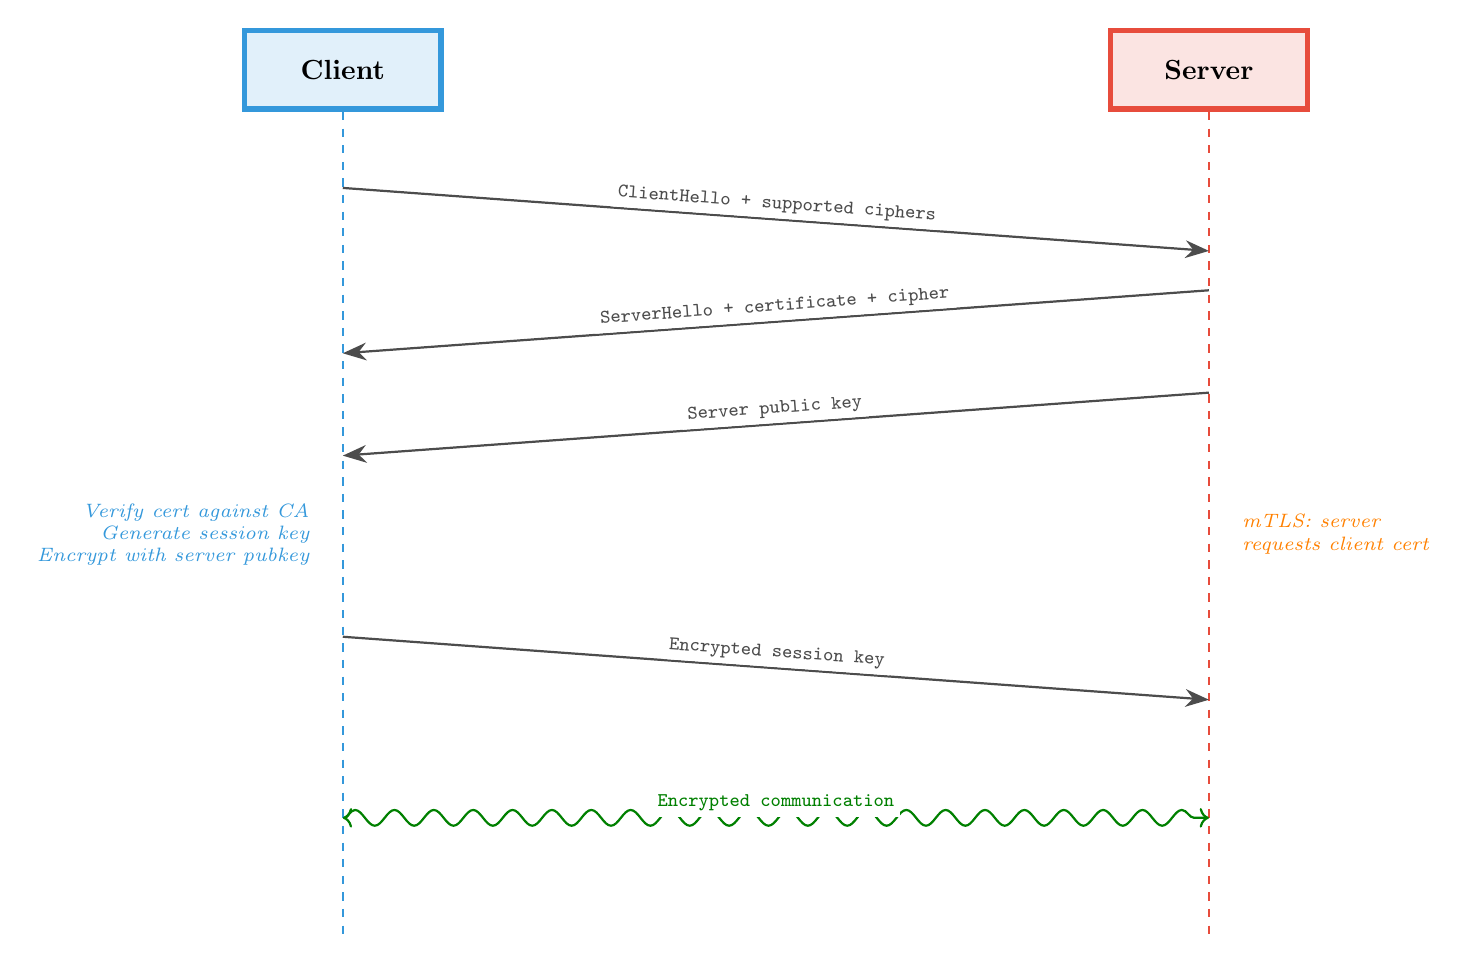
\begin{tikzpicture}[
        entity/.style={rectangle, draw=#1, fill=#1!15, line
        width=2pt, minimum width=2.5cm, minimum height=1cm, font=\bfseries},
        msg/.style={-{Stealth[length=3mm]}, thick, black!70},
        msglabel/.style={font=\scriptsize\ttfamily, fill=white, inner sep=2pt},
        note/.style={font=\scriptsize\itshape, text=peer},
      ]
      \node[entity=peer] (clt) at (0, 0) {Client};
      \node[entity=router] (srv) at (11, 0) {Server};

      \draw[thick, peer, dashed] (clt.south) -- ++(0, -10.5);
      \draw[thick, router, dashed] (srv.south) -- ++(0, -10.5);

      \draw[msg] (0, -1.5) -- node[msglabel, above, sloped]
      {ClientHello + supported ciphers} (11, -2.3);
      \draw[msg] (11, -2.8) -- node[msglabel, above, sloped]
      {ServerHello + certificate + cipher} (0, -3.6);
      \draw[msg] (11, -4.1) -- node[msglabel, above, sloped] {Server
      public key} (0, -4.9);

      \node[note, anchor=east, align=right] at (-0.3, -5.9) {Verify
      cert against CA\\Generate session key\\Encrypt with server pubkey};

      \draw[msg] (0, -7.2) -- node[msglabel, above, sloped]
      {Encrypted session key} (11, -8.0);

      \node[font=\scriptsize\itshape, text=orange, anchor=west,
      align=left] at (11.3, -5.9) {mTLS: server\\requests client cert};

      \draw[msg, <->, green!50!black, decorate, decoration={snake,
      amplitude=1mm, segment length=5mm}]
      (0, -9.5) -- node[msglabel, above] {Encrypted communication} (11, -9.5);
    \end{tikzpicture}
  \end{adjustbox}
  \caption{The TLS handshake. In mutual TLS, the server also requests
  a certificate from the client.}
  \label{fig:tls}
\end{figure}

In standard TLS, only the server proves its identity. In mutual TLS
(mTLS), the server also requests a certificate from the client. Both
sides verify each other's certificate against the same Certificate
Authority. This matters for the DVerse platform because it ensures
that both endpoints are authenticated members of the platform, not
just that the connection is encrypted. Zenoh enables mTLS through the
\texttt{enable\_mtls} configuration flag~\citep{zenoh-tls,zenoh-config}.

\subsection{Certificates and Issuance}

A certificate binds a public key to an identity. Certificates are
issued by a Certificate Authority (CA) that both parties
trust~\citep{rfc5280}. Anyone who has the CA's root certificate can
verify that a given certificate was issued legitimately.
Figure~\ref{fig:certs} illustrates this.

\begin{figure}[H]
  \centering
  \begin{adjustbox}{max width=\textwidth}
    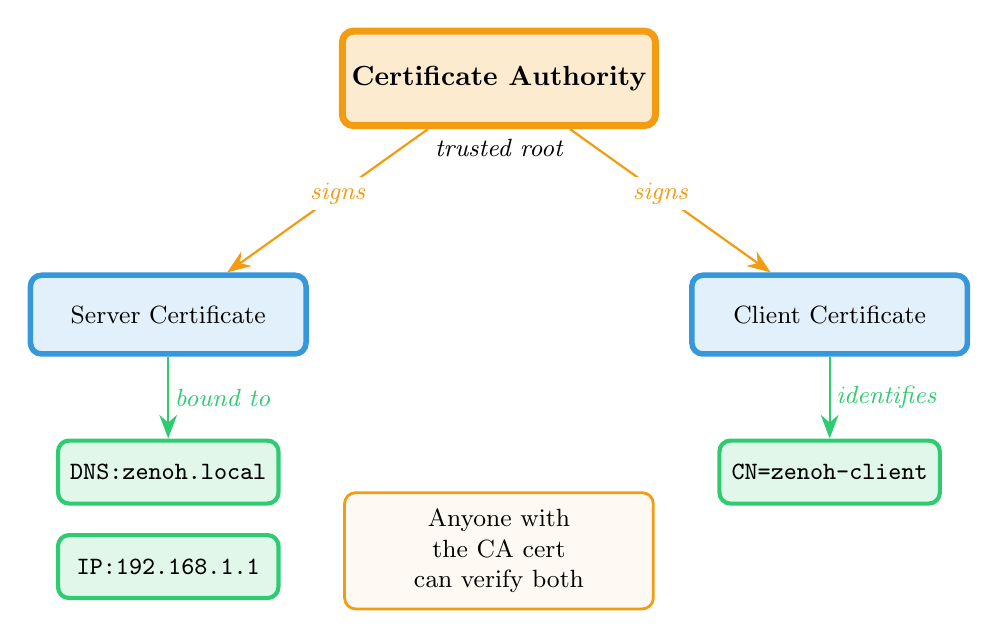
\begin{tikzpicture}[
        authority/.style={rectangle, rounded corners, draw=ca,
          fill=ca!20, line width=2.5pt, minimum width=3cm, minimum
        height=1.2cm, font=\bfseries},
        certnode/.style={rectangle, rounded corners, draw=cert,
          fill=cert!15, line width=2pt, minimum width=3.5cm, minimum
        height=1cm, font=\small},
        domnode/.style={rectangle, rounded corners, draw=domaincol,
          fill=domaincol!15, line width=1.5pt, minimum width=2.8cm,
        minimum height=0.8cm, font=\small\ttfamily},
        arr/.style={-{Stealth[length=3mm]}, thick},
        signlabel/.style={font=\small\itshape, fill=white, inner sep=2pt},
      ]
      \node[authority] (canode) at (0, 0) {Certificate Authority};
      \node[font=\small\itshape, anchor=north] at (canode.south) {trusted root};

      \node[certnode] (servercert) at (-4.2, -3) {Server Certificate};
      \node[certnode] (clientcert) at (4.2, -3) {Client Certificate};

      \draw[arr, ca] (canode) -- node[signlabel, pos=0.45] {signs} (servercert);
      \draw[arr, ca] (canode) -- node[signlabel, pos=0.45] {signs} (clientcert);

      \node[domnode] (dns) at (-4.2, -5) {DNS:zenoh.local};
      \node[domnode] (ip) at (-4.2, -6.2) {IP:192.168.1.1};

      \draw[arr, domaincol] (servercert) -- node[signlabel, right,
      pos=0.5] {bound to} (dns);

      \node[domnode] (cn) at (4.2, -5) {CN=zenoh-client};
      \draw[arr, domaincol] (clientcert) -- node[signlabel, right,
      pos=0.5] {identifies} (cn);

      \node[rectangle, rounded corners, draw=ca, fill=ca!5, line
        width=1pt, inner sep=6pt, font=\small, align=center, text
      width=3.5cm] at (0, -6) {Anyone with the CA cert\\can verify both};
    \end{tikzpicture}
  \end{adjustbox}
  \caption{Certificate issuance. The CA signs both server and client
  certificates.}
  \label{fig:certs}
\end{figure}

Certificates are issued to a specific identity: either a DNS name
such as \texttt{zenoh.local}, or an IP address. This identity is
encoded in the certificate's Subject Alternative Name (SAN)
field~\citep{rfc5280}. During a TLS handshake, the connecting party
verifies that the SAN matches the address it connected to. Zenoh can
verify the match between hostname and certificate via the
\texttt{verify\_name\_on\_connect} setting, which is enabled by
default~\citep{zenoh-config}.

A key finding during the evaluation was the importance of the
Extended Key Usage (EKU) field defined in~\citep{rfc5280}. Server
certificates must have the \texttt{serverAuth} EKU, and client
certificates must have the \texttt{clientAuth} EKU. Without the
correct EKU, Zenoh's TLS implementation rejects the connection with a
\texttt{BadCertificate} error, even if the certificate chain is valid
and verified.

\subsection{Enforcing TLS-Only Communication in Zenoh}

A critical finding is that configuring TLS certificates in Zenoh does
not, by itself, prevent unauthenticated connections. Zenoh's TLS
configuration only activates when a connection uses the \texttt{tls/}
protocol scheme. If the router also listens on \texttt{tcp/},
unauthenticated clients can connect over plain TCP and bypass TLS
entirely. The Zenoh documentation addresses this directly by
recommending the \texttt{protocols} whitelist in the transport link
configuration~\citep{zenoh-tls}.

In the same way, Zenoh's scouting mechanism lets nodes discover each
other via multicast UDP on group \texttt{224.0.0.224} port
\texttt{7446}~\citep{zenoh-deployment}. Scouting operates outside the
TLS layer, so an unauthenticated node can join the network through
scouting even if all configured endpoints use TLS.

To enforce TLS-only communication, two measures are required. First,
the router must only expose \texttt{tls/} listen endpoints; no
\texttt{tcp/} listeners should be configured. Second, all scouting
(both multicast and gossip) must be disabled so that nodes must
connect through explicitly configured endpoints
only~\citep{zenoh-config,zenoh-deployment}.

The router listen endpoint was set to \texttt{tls/[::]:7447} to
accept connections on both IPv4 and IPv6. On Linux, binding to
\texttt{[::]} covers both address families by default when the
\path{net.ipv6.bindv6only} sysctl is \texttt{0}, which is the
standard setting. This was necessary because mDNS name resolution can return
either an IPv4 or IPv6 address depending on the network configuration.

\subsection{Configuration}

The router runs in \texttt{router} mode with scouting disabled and
only a TLS listener, as shown in Listing~\ref{lst:router}. Client
nodes connect in \texttt{client} mode with their own certificate
pair, as shown in Listing~\ref{lst:client}. The field names follow
the conventions documented in Zenoh 1.0
``Firesong''~\citep{zenoh-firesong,zenoh-config}.

\begin{lstlisting}[language=Java,caption={Router configuration (JSON5).},label={lst:router}]
{
  mode: "router",
  listen: { endpoints: ["tls/[::]:7447"] },
  scouting: {
    multicast: { enabled: false },
    gossip: { enabled: false }
  },
  transport: {
    link: {
      tls: {
        root_ca_certificate: "./certs/ca.crt",
        listen_private_key: "./certs/server.key",
        listen_certificate: "./certs/server.crt",
        enable_mtls: true
      }
    }
  }
}
\end{lstlisting}

\begin{lstlisting}[language=Java,caption={Client configuration (JSON5).},label={lst:client}]
{
  mode: "client",
  connect: { endpoints: ["tls/zenoh.local:7447"] },
  scouting: { multicast: { enabled: false } },
  transport: {
    link: {
      tls: {
        root_ca_certificate: "./certs/ca.crt",
        connect_private_key: "./certs/client.key",
        connect_certificate: "./certs/client.crt",
        enable_mtls: true
      }
    }
  }
}
\end{lstlisting}

% ==============================================================
\section{V3 Findings: Why Static ACLs Were Not Enough}
\label{sec:v3-acls}
% ==============================================================

The V2 design landed at a fabric that authenticates every node via
mTLS and intended to layer a session-level ACL on top of that fabric
to keep cert holders out of sessions they had not been admitted to.
The implementation work in V3 attempted exactly that. It surfaced a
property of Zenoh's ACL model that the V2 plan had not anticipated:
the ACL configuration is consumed once, when the Zenoh session is
opened, and there is no API to mutate it afterwards. This section
records the finding, the cost it imposes on a dynamic system, and the
design that replaced it.

\subsection{The Reload Problem}

A Zenoh \texttt{Session} is constructed from a \texttt{Config} that
contains the full ACL JSON. The runtime reads this configuration
during \texttt{zenoh::open(config)}: the allow and deny rules, the
subject definitions, and the per-rule key expressions are compiled
into the session's routing tables once and then frozen for the
lifetime of the session~\citep{zenoh-acl,zenoh-acl-rfc}. There is no
\texttt{Session::reload\_acls()} call, no in-place mutation of the
admitted-CN list, and no upstream RFC promising one.

For a system where the admitted set changes during normal operation,
this is a binding constraint. The DVerse admin is expected to accept
or deny join requests at runtime, and every such decision has to
propagate to the data plane. With static ACLs, propagating a decision
means rebuilding the session: discard the current
\texttt{Session}, construct a new \texttt{Config} with the updated
admitted list, call \texttt{zenoh::open} again, and re-declare every
publisher and subscriber the router was running.

In the implementation in
\texttt{src/zenoh\_router/src/router.rs}, this manifests as the outer
\texttt{run()} loop. The inner \texttt{session\_loop} returns whenever
the admitted set or the staged session config changes. The router
then aborts the admission handler and the periodic republish task,
closes the existing Zenoh session, marks itself
\texttt{RouterStatus::Reloading}, and iterates the outer loop. The
next iteration rebuilds the ACL JSON from the new admitted list,
opens a fresh session, and re-declares every subscription. While that
happens, the router is genuinely down on the wire: no agent payload
gets through.

That window is the cost. It is invisible in unit tests because the
test fixture admits everyone before the session opens. It is visible
under any realistic admission workload: every accept and every deny
incurs a session rebuild on the host that drove the change, and the
agents on that host see a brief outage. Continuous availability,
which is the property the platform exists to provide, is violated
each time a member joins or leaves.

\subsection{The Pivot: Admission Handshake plus Megolm}

V3 replaces the ``ACL edit per join'' design with a two-layer model:

\begin{itemize}[leftmargin=1.4em]
  \item A single broad allow rule for \texttt{dverse/**} scoped to the
        currently admitted CNs. This rule still lives in the static
        ACL JSON, but it is now expected to be rebuilt only on real
        membership changes (an admit or a deny), not on every action
        an admitted member takes. The ACL has become a coarse
        fabric-level gate, not the fine-grained access control
        mechanism.
  \item A cryptographic membership check layered above the fabric.
        Admission is a handshake on a pair of well-known Zenoh
        topics. The requester publishes a signed \texttt{JoinRequest}
        carrying its mDNS-discovered CN, its vodozemac Curve25519
        identity key, an Ed25519 fingerprint, a one-time prekey, and
        an ECDSA P-256 signature binding the encryption key to the
        cert. The admin verifies the signature against the
        requester's leaf certificate, then publishes an
        \texttt{AdmissionDecision::Allow} that contains the admin's
        Megolm \texttt{SessionKey} encrypted with an Olm pre-key
        message addressed to the requester's one-time key. Only the
        requester, who holds the matching private key, can decrypt
        the wrap and install the \texttt{GroupReceiver}.
\end{itemize}

Once the requester has installed the receiver, it is part of the
session at the cryptographic layer regardless of what the ACL does.
Every agent payload is encrypted with Megolm before it goes on the
wire. A peer that holds a valid DVerse cert but does not hold the
session key sees opaque ciphertext on every topic; the topic itself
is allowed by the broad fabric rule, but the data is not legible.

\subsection{Cross-Machine Key Distribution}

Megolm gives each agent process a per-process outbound
\texttt{SessionKey} that other agents have to install as a
\texttt{GroupReceiver} before they can decrypt the agent's messages.
The same-machine case is easy: every agent writes its key to a
shared filesystem directory under \texttt{<cert\_dir>/megolm/} and
peers pick it up on the next refresh tick. The cross-machine case
needs more work, because agents on different operators never see each
other's filesystems.

V3 ships a wire-relay alongside the filesystem mechanism. Each agent
runs a small background task that publishes its session key on
\texttt{dverse/agent\_keys/<cn>/<agent\_name>} every five seconds,
and a subscriber on \texttt{dverse/agent\_keys/**} that calls
\texttt{install\_peer\_session\_key} for each envelope it receives.
The install routine skips envelopes whose session id matches the
local sender (a node never installs a receiver against its own
sender, which would corrupt outbound ordering) and is idempotent on
re-installation of an already-known peer. The relay topic falls
under the same broad fabric rule that protects every other
\texttt{dverse/**} expression: only admitted CNs see it. The security
boundary on key distribution is therefore the admission decision, not
a separate ACL rule.

\subsection{Why This Is a Better Fit}

The cost of an admission decision under V3 is one admitted-list
update (which still rebuilds the session, but membership changes are
now the common case, not the every-message case) plus a one-shot Olm
encrypt on the admin and an Olm decrypt on the requester. Installing
a peer's Megolm receiver is an in-memory \texttt{HashMap} insert. The
admitted-list-change latency, qualitatively:

\begin{table}[H]
  \centering
  \small
  \begin{tabular}{|p{4.4cm}|p{3.4cm}|p{6.4cm}|}
    \hline
    \rowcolor{gray!15}
    \textbf{Event} & \textbf{V2 static ACL} & \textbf{V3 admission + crypto} \\
    \hline
    Admit a CN & session rebuild & ACL rewrite + Olm wrap + \texttt{HashMap::insert} on the requester \\
    \hline
    Agent A learns about agent B's key & N/A (no payload crypto) & relay tick (worst case 5\,s, typical $<$1\,s) \\
    \hline
    Per-payload encryption cost & none & Megolm AEAD seal/open \\
    \hline
    In-flight payloads during a swap & lost & lost only for the brief swap window; receivers persist across swaps \\
    \hline
  \end{tabular}
  \caption{Cost shape of admission events under V2 versus V3.}
  \label{tab:v2v3}
\end{table}

The crypto layer is hot-updatable by construction. Throughput
continues across joins because the data plane does not pause when a
new \texttt{GroupReceiver} appears in the map.

\subsection{The Mid-Run Session Swap Doorbell}

There is still one operation in V3 that genuinely needs the
fabric-level rebuild: an operator logging out of one session and
joining another. The role of the local router flips between admin and
client, and the namespace under which Zenoh runs changes. That cannot
be done by editing in-memory state alone; the Zenoh session is built
for one namespace, and the new namespace requires
\texttt{zenoh::open} to run against a new \texttt{Config}.

The router state therefore exposes two notification doorbells
(each an \path{Arc<tokio::sync::Notify>}). The first,
\texttt{admitted\_changed}, is rung by the admission handler after a
successful admit or deny so the inner loop returns and the outer
loop rebuilds the ACL. The second, \texttt{config\_changed}, is rung
by the Tauri command that stages a new session config. When a user
picks a different session from the chooser screen, the launcher
writes the new \texttt{DverseConfig} into \texttt{staged\_config} on
the router state and calls \texttt{config\_changed.notify\_one()}.
The inner \texttt{session\_loop} returns immediately, and Phase~1 of
the outer loop prefers the freshly staged config over any cached one.

That last detail is worth recording because it was a regression in
an earlier V3 iteration. The first cut consulted
\texttt{staged\_config} only on the router's first boot; subsequent
session restarts silently reused the previously-cached
\texttt{current\_cfg}. Switching sessions appeared to work in the UI
but the router carried on under the old role. The fix consumes
\texttt{staged\_config} on every iteration of the outer loop and
wipes per-session state (crypto, admitted list, pending requests,
mDNS announcer) when a fresh config is consumed. Without that change,
the doorbell would still be rung but the new role would not take
effect.

The general lesson is that V2's static-ACL design quietly leaked into
operations even after the V3 crypto layer was in place. The role of
the broad fabric rule is now narrow enough that a session rebuild is
an exceptional event, not a per-action one. The remaining work is
ensuring the operational machinery agrees.

\subsection{The Keycloak + OIDC + Step-CA enrolment pipeline}
\label{sec:oidc-pipeline}

V3 needed every operator and every agent to hold a short-lived
TLS leaf cert signed by a trust root that the dverse fabric agrees
on. V2 imagined this happening through an offline ``the operator
emails the admin a CSR'' workflow, which does not scale and does
not tie the cert to a real-world identity. V3 replaced that with a
self-service enrolment pipeline driven by an OIDC identity provider.
Figure~\ref{fig:oidc-flow} sketches the round-trip.

\begin{figure}[H]
\centering
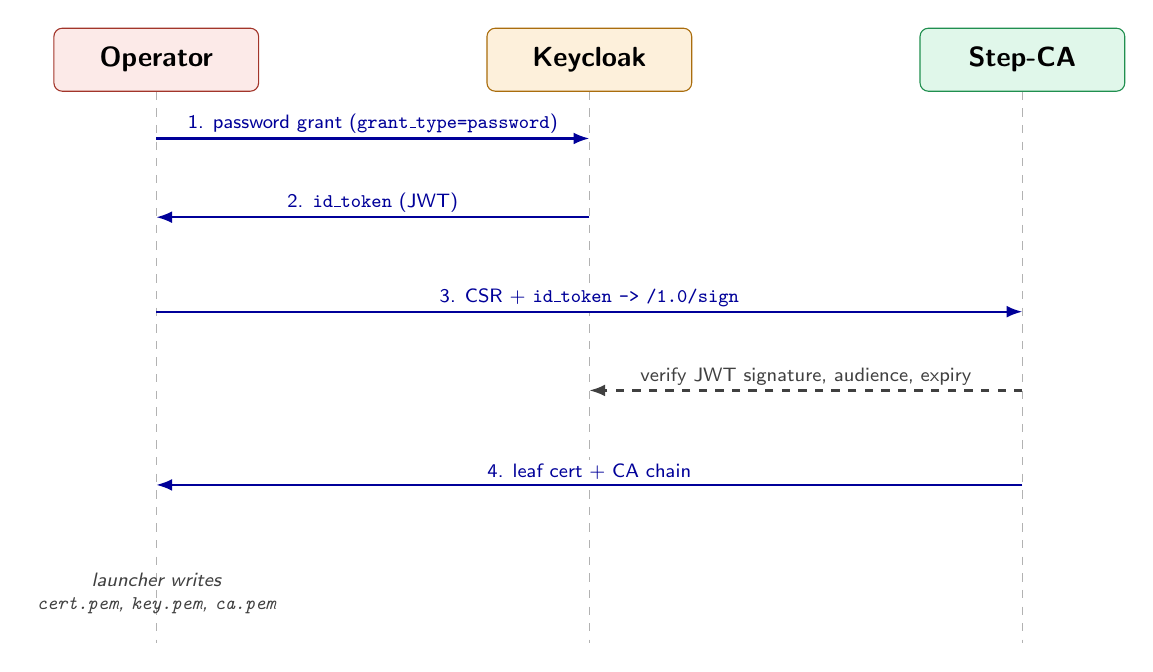
\begin{tikzpicture}[
  every node/.style={font=\sffamily\footnotesize},
  actor/.style={
    draw=router!70!black, fill=router!12, rounded corners=3pt,
    minimum width=2.6cm, minimum height=0.8cm, align=center,
    inner sep=3pt, font=\sffamily\bfseries,
  },
  kcbox/.style={
    draw=ca!70!black, fill=ca!15, rounded corners=3pt,
    minimum width=2.6cm, minimum height=0.8cm, align=center,
    inner sep=3pt, font=\sffamily\bfseries,
  },
  cabox/.style={
    draw=admitted!70!black, fill=admitted!15, rounded corners=3pt,
    minimum width=2.6cm, minimum height=0.8cm, align=center,
    inner sep=3pt, font=\sffamily\bfseries,
  },
  life/.style={dashed, gray!60},
  msg/.style={-{Latex[length=2mm]}, thick, blue!60!black},
  vmsg/.style={-{Latex[length=2mm]}, thick, dashed, gray!50!black},
  lbl/.style={font=\scriptsize\sffamily, fill=white, inner sep=1.5pt, midway},
]
  % Three actors with vertical lifelines
  \node[actor] (op) at (0, 0)   {Operator};
  \node[kcbox] (kc) at (5.5, 0) {Keycloak};
  \node[cabox] (ca) at (11, 0)  {Step-CA};

  \draw[life] (op.south) -- ++(0, -7);
  \draw[life] (kc.south) -- ++(0, -7);
  \draw[life] (ca.south) -- ++(0, -7);

  % Sequence (top to bottom, evenly spaced)
  \draw[msg] (op.south |- 0,-1.0) -- (kc.south |- 0,-1.0)
    node[lbl, above]{1. password grant (\texttt{grant\_type=password})};
  \draw[msg] (kc.south |- 0,-2.0) -- (op.south |- 0,-2.0)
    node[lbl, above]{2. \texttt{id\_token} (JWT)};
  \draw[msg] (op.south |- 0,-3.2) -- (ca.south |- 0,-3.2)
    node[lbl, above]{3. CSR + \texttt{id\_token} \texttt{->} \texttt{/1.0/sign}};
  \draw[vmsg] (ca.south |- 0,-4.2) -- (kc.south |- 0,-4.2)
    node[lbl, above]{verify JWT signature, audience, expiry};
  \draw[msg] (ca.south |- 0,-5.4) -- (op.south |- 0,-5.4)
    node[lbl, above]{4. leaf cert + CA chain};

  % Small annotation under operator showing what's written to disk
  \node[font=\scriptsize\sffamily\itshape, text=gray!50!black,
        anchor=north, align=center]
    at (op.south |- 0,-6.4)
    {launcher writes\\\texttt{cert.pem}, \texttt{key.pem}, \texttt{ca.pem}};
\end{tikzpicture}
\caption{The V3 enrolment pipeline as a sequence. The launcher
exchanges Keycloak credentials for an OIDC \texttt{id\_token},
sends a freshly-generated CSR plus the token to Step-CA, and
Step-CA returns a short-lived leaf certificate after verifying the
token against Keycloak's published OIDC configuration.}
\label{fig:oidc-flow}
\end{figure}

The pieces, in the order the launcher exercises them:

\subsubsection{Keycloak as the identity provider}
A Keycloak instance runs on the dverse trust-root host (the VPS
described in the companion \emph{Nix} portfolio document). It holds
the user database and the realm configuration; operators and agents
have accounts under email addresses like
\texttt{<name>@dverse.yordanmitev.me}. A dedicated OIDC client is
registered in the realm for Step-CA enrolment, with its own client
ID and client secret.

\subsubsection{Step-CA as the signing service}
Step-CA runs on the same trust-root host, configured with an OIDC
provisioner that points at Keycloak's OIDC discovery endpoint. The
provisioner's settings declare the allowed audience and the
template that determines what goes into the issued certificate.
The Step-CA template, in the deployed configuration, sets:

\begin{itemize}[leftmargin=1.4em]
  \item \textbf{CN} = the username portion of the email
        (\texttt{<name>@dverse.yordanmitev.me} $\rightarrow$
        CN = \texttt{<name>}). This is the identity that the
        admission handshake of Section~\ref{sec:v3-acls} verifies.
  \item \textbf{SAN} = the full email address \emph{and}
        \texttt{zenoh-<name>.local}. The \texttt{.local} SAN is
        what the mDNS discovery of Section~\ref{sec:mdns} resolves to,
        so TLS validation against a peer found over mDNS will
        succeed.
\end{itemize}

\subsubsection{The launcher's role}
At login, the launcher POSTs the operator's Keycloak username and
password to the realm's OIDC token endpoint
(\path{/realms/<realm>/protocol/openid-connect/token}) with the
\texttt{password} grant type, the registered client ID and secret,
and the \texttt{openid} scope. It receives an \texttt{id\_token}
(a JWT) back, then generates a fresh key pair with the
\texttt{rcgen}~\citep{rcgen} crate, builds a CSR, and POSTs both
to Step-CA's \texttt{/1.0/sign} endpoint as
\texttt{\{csr, ott\}} (Step-CA names the token \texttt{ott},
``one-time token''). Step-CA validates the JWT signature against
Keycloak's published JWKS, checks the audience and expiry, applies
the certificate template, and returns the signed cert plus the
issuing CA chain. The launcher writes the three resulting files
(\texttt{cert.pem}, \texttt{key.pem}, \texttt{ca.pem}) to the
operator's configured certificate directory.

\subsubsection{Agent enrolment}
The demo agents (\texttt{ping}, \texttt{pong}, and any future agent
in the workspace) acquire their own certificates through the same
flow at first launch, using a service-account credential that the
operator's setup provides. The CN of an agent's cert encodes the
agent's role (\texttt{ping}, \texttt{pong}) so the per-agent
identity is visible in the published mDNS records and in the
admission decisions.

\subsubsection{Rotation}
Certificates issued under this template have a short lifetime (the
demo configuration uses 24 hours). Each process checks at startup
whether its on-disk cert is within a renewal window
(\texttt{cert::needs\_renewal}, default 23 hours of the 24-hour
lifetime) and, if so, walks the same Keycloak~$\rightarrow$~Step-CA
flow to acquire a fresh one. The result is that revocation is
effectively automatic on the next renewal window: removing a user
from Keycloak's realm means their next enrolment fails, and within
a day their cert has expired and no replacement is forthcoming.

\subsubsection{How this ties into V3 admission}
The TLS handshake gates whether a node can connect to the fabric
at all; the admission handshake gates whether a CN gets a Megolm
\texttt{SessionKey} for a specific session
(Section~\ref{sec:v3-acls}). The pipeline above is what binds a
real-world identity (a Keycloak account) to the CN that those two
gates check. If the trust-root host disappears, no new certificates
can be issued, but existing operators continue to function until
their cert expires --- the fabric is not online-only.

% ==============================================================
\section{Local Node Discovery with mDNS}
\label{sec:mdns}
% ==============================================================

A key challenge in a decentralized system is how nodes find each
other on the local network without hardcoding IP addresses. Zenoh's
built-in scouting over multicast UDP cannot be used because it
bypasses TLS and would let unauthenticated nodes discover and join
the network.

The solution is mDNS / DNS-SD (Multicast DNS with service discovery),
specified in RFC~6762~\citep{rfc6762} and RFC~6763. The V2 plan
called for using the system-level Avahi daemon~\citep{avahi} to
publish each machine's \texttt{.local} hostname; V3 changed this
(see Section~\ref{sec:mdns-mdnssd}) and embedded discovery inside the
operator process via the \texttt{mdns-sd} Rust
crate~\citep{mdnssd}, removing the need for a system daemon.

\subsection{How mDNS Works}

The \texttt{.local} top-level domain is reserved for link-local
multicast name resolution~\citep{rfc6762}. When a machine needs to
resolve a \texttt{.local} hostname, it sends a multicast query to
address \texttt{224.0.0.251} on UDP port \texttt{5353} (or the IPv6
equivalent \texttt{FF02::FB}). The machine that owns that hostname
responds with its IP address. No DNS server is involved.

The same multicast channel carries DNS-SD service records, which let
a node not just look up a name but \emph{browse} for services
matching a service type (for example, \texttt{\_dverse.\_tcp.local}).
V3 uses this browse capability so that one operator's launcher
discovers every other operator's session without prior knowledge of
hostnames.

On Linux mDNS is most commonly implemented by the Avahi
daemon~\citep{avahi}; on macOS by Bonjour; on Windows it is native
since Windows 10 1903~\citep{ms-mdns}. mDNS is distinct from LLMNR
(RFC~4795~\citep{rfc4795}); the two protocols are not compatible
(different port \texttt{5355}, different multicast address, and LLMNR
is typically single-label only). Microsoft has been phasing out
LLMNR in favour of mDNS~\citep{ms-mdns}, so targeting mDNS provides
the best cross-platform coverage today.

\subsection{V3: \texttt{mdns-sd} embedded in the operator process}
\label{sec:mdns-mdnssd}

The V2 design assumed each machine ran a system-level Avahi daemon
configured through \texttt{/etc/avahi/avahi-daemon.conf}. In
practice this turned out to be a poor fit for the dverse use case:
Avahi is a host-level service whose advertisements are visible to
every process on the machine, advertises on every interface unless
configured otherwise (so Docker bridge networks routinely leak into
the hostname-to-IP mapping), and requires elevated privileges and
distribution-specific setup that the operator should not have to
care about.

V3 dropped Avahi entirely. The Rust crate
\texttt{mdns-sd}~\citep{mdnssd} provides a pure-Rust mDNS + DNS-SD
implementation: it opens the multicast socket on a configured
interface, sends and answers queries directly, and exposes a
\texttt{ServiceDaemon::register} call for advertising a service and
a \texttt{browse} call for discovering peers. The operator's router
process embeds the crate, registers its own session under the
\texttt{\_dverse.\_tcp.local} service type with the operator's CN as
a TXT record, and concurrently browses the same type to populate
the chooser screen in the launcher.

The benefits of moving discovery in-process:

\begin{itemize}[leftmargin=1.4em]
  \item \textbf{Scoped advertisements.} The advertisement and the
        browse both happen on the interface the operator's router
        actually listens on, with no risk of Docker bridges or
        unrelated interfaces being included.
  \item \textbf{No system service.} No \texttt{avahi-daemon} to
        install, configure, or troubleshoot; the launcher works
        identically on Linux, macOS, and Windows.
  \item \textbf{Lifecycle bound to the operator.} The
        advertisement disappears the moment the router exits;
        there is no stale entry from a previous run lingering until
        the next system reboot.
  \item \textbf{Direct access to TXT records.} The CN goes into a
        \texttt{cn=} TXT entry rather than being parsed out of a
        full mDNS service-instance name; this is how the launcher
        knows which CN to address its \texttt{JoinRequest} to.
\end{itemize}

\subsection{Certificate Integration}

Because the mDNS hostname is stable and independent of the
machine's IP address, the operator's TLS certificate is issued with
\texttt{DNS:zenoh-<username>.local} as the SAN, where
\texttt{<username>} is the operator's Keycloak username portion
(see Section~\ref{sec:oidc-pipeline}). TLS validation succeeds regardless
of which IP address the machine currently has, because the
certificate's SAN matches the same mDNS-published name that the
peer just resolved.

% ==============================================================
\section{Platform Architecture}
% ==============================================================

Based on the TLS and discovery findings, the architecture shown in
Figure~\ref{fig:architecture} has been designed and validated for the
DVerse platform. As a reminder, the scope of this document is the
communication and security layer. How individual agents are
constructed, what their internal behavior is, and what
application-level APIs they expose are separate concerns that will be
documented elsewhere once their design is clearer.

\begin{figure}[H]
  \centering
  \begin{adjustbox}{max width=\textwidth}
    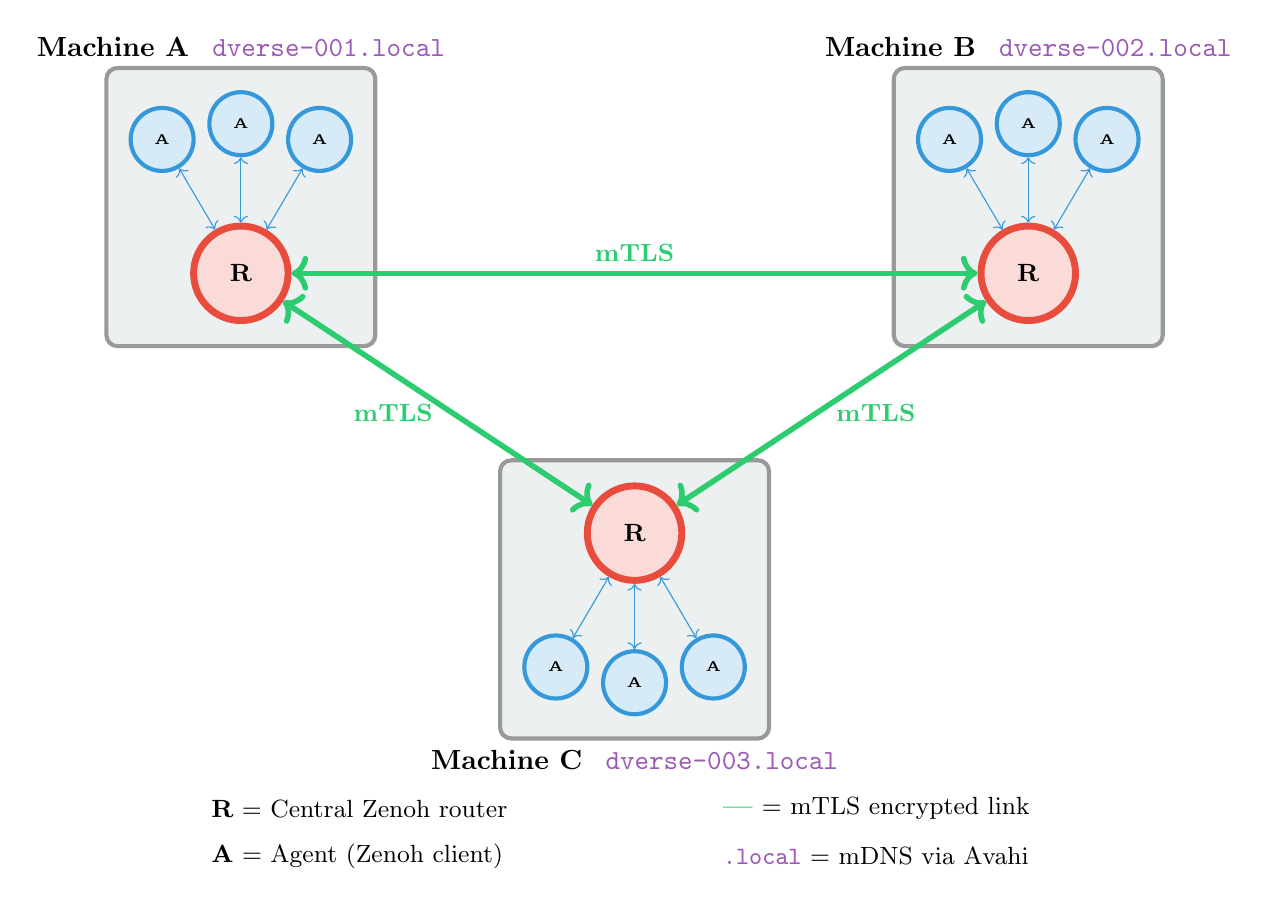
\begin{tikzpicture}[
        routernode/.style={circle, draw=router, fill=router!20, line
        width=2.5pt, minimum size=1.2cm, font=\bfseries\small},
        agentnode/.style={circle, draw=agent, fill=agent!20, line
        width=1.5pt, minimum size=0.8cm, font=\bfseries\tiny},
        machinebox/.style={rectangle, rounded corners, draw=black!40,
        fill=machine, line width=1.5pt, inner sep=8pt},
        tlslink/.style={<->, thick, tls, line width=2pt},
        locallink/.style={<->, thin, agent},
      ]
      % Machine A (top left) - agents ON TOP, router at the bottom of the box
      \node[agentnode] (a1) at (-1.0, 0) {A};
      \node[agentnode] (a2) at (0, 0.2) {A};
      \node[agentnode] (a3) at (1.0, 0) {A};
      \node[routernode] (r1) at (0, -1.7) {R};
      \draw[locallink] (r1) -- (a1);
      \draw[locallink] (r1) -- (a2);
      \draw[locallink] (r1) -- (a3);
      \begin{scope}[on background layer]
        \node[machinebox, fit=(r1)(a1)(a2)(a3)] (m1) {};
      \end{scope}
      \node[anchor=south] at (m1.north) {\textbf{Machine A} \,
      \textcolor{avahi}{\ttfamily dverse-001.local}};

      % Machine B (top right) - agents ON TOP, router at the bottom
      \node[agentnode] (b1) at (9.0, 0) {A};
      \node[agentnode] (b2) at (10, 0.2) {A};
      \node[agentnode] (b3) at (11.0, 0) {A};
      \node[routernode] (r2) at (10, -1.7) {R};
      \draw[locallink] (r2) -- (b1);
      \draw[locallink] (r2) -- (b2);
      \draw[locallink] (r2) -- (b3);
      \begin{scope}[on background layer]
        \node[machinebox, fit=(r2)(b1)(b2)(b3)] (m2) {};
      \end{scope}
      \node[anchor=south] at (m2.north) {\textbf{Machine B} \,
      \textcolor{avahi}{\ttfamily dverse-002.local}};

      % Machine C (bottom center) - router ON TOP, agents at the
      % bottom of the box
      \node[routernode] (r3) at (5, -5) {R};
      \node[agentnode] (c1) at (4.0, -6.7) {A};
      \node[agentnode] (c2) at (5, -6.9) {A};
      \node[agentnode] (c3) at (6.0, -6.7) {A};
      \draw[locallink] (r3) -- (c1);
      \draw[locallink] (r3) -- (c2);
      \draw[locallink] (r3) -- (c3);
      \begin{scope}[on background layer]
        \node[machinebox, fit=(r3)(c1)(c2)(c3)] (m3) {};
      \end{scope}
      \node[anchor=north] at (m3.south) {\textbf{Machine C} \,
      \textcolor{avahi}{\ttfamily dverse-003.local}};

      % Direct router-to-router mTLS links
      \draw[tlslink] (r1) -- node[above, font=\small\bfseries,
      text=tls] {mTLS} (r2);
      \draw[tlslink] (r1) -- node[left=3pt, font=\small\bfseries,
      text=tls, pos=0.55] {mTLS} (r3);
      \draw[tlslink] (r2) -- node[right=3pt, font=\small\bfseries,
      text=tls, pos=0.55] {mTLS} (r3);

      % Legend
      \node[font=\small, anchor=west] at (-0.5, -8.5) {\textbf{R} =
      Central Zenoh router};
      \node[font=\small, anchor=west] at (-0.5, -9.1) {\textbf{A} =
      Agent (Zenoh client)};
      \node[font=\small, anchor=west] at (6, -8.5)
      {{\color{tls}\textbf{---}} = mTLS encrypted link};
      \node[font=\small, anchor=west] at (6, -9.1)
      {{\color{avahi}\texttt{.local}} = mDNS via Avahi};
    \end{tikzpicture}
  \end{adjustbox}
  \caption{The DVerse platform architecture. Each machine runs a
    central Zenoh router with local agents connecting as clients.
  Routers form an mTLS mesh, discovered via mDNS.}
  \label{fig:architecture}
\end{figure}

Each physical machine runs one central Zenoh router. This router
listens on TLS and acts as the hub for all agents running on that
machine. Agents connect to the local router as Zenoh clients over
TLS. They never communicate directly with the outside network. All
inter-machine communication flows through the router mesh.

Routers on different machines connect to each other over mTLS,
forming a mesh. Each router has a unique \texttt{dverse-<id>.local}
hostname advertised via Avahi~\citep{avahi}, and its server
certificate is issued for that hostname. Routers can find each other
on the local network by name and establish authenticated, encrypted
links without any centralized coordination.

\subsection{The Central Router is Not Just \texttt{zenohd}}

The central Zenoh router in this architecture is not a plain
\texttt{zenohd} process. It runs the Zenoh routing stack together
with a small administrative API. This API is responsible for the
session-level decisions that Zenoh itself does not handle.
Specifically, the API supports operations such as admitting a new
router into the session, denying a pending request, banning a
previously admitted router, and listing currently connected routers.

The API runs alongside the Zenoh router on the same process or the
same machine. It reads admittance requests from the Zenoh topic space
(see Section~\ref{sec:v3-acls}) and writes decisions back through
Zenoh's ACL configuration~\citep{zenoh-acl,zenoh-acl-rfc}. By keeping
this logic on the central router, each machine remains in control of
which other machines it trusts, without relying on a central coordinator.

\subsection{Certificate Strategy}

The certificate strategy is designed around a cloud-hosted CA. When a
new machine is registered with the platform, the cloud CA issues
three things. First, a server certificate bound to the machine's
\texttt{dverse-<id>.local} hostname, with the \texttt{serverAuth}
EKU. Second, client certificates for the agents running on that
machine, with the \texttt{clientAuth} EKU. Third, the CA root
certificate, distributed to all nodes so they can verify each other.

This keeps certificate management centralized while the actual
communication stays fully decentralized. A machine can be added to
the platform by registering it, receiving its certificates, and
starting the Zenoh router. No changes to any other machine are required.

% ==============================================================
\section{Testing the Security Layer}
\label{sec:testing}
% ==============================================================

This section is deliberately small. It records what is verified
by unit tests today, where those tests live, and the
relationship to the existing chat-app CI pipeline that informed
the team's testing discipline.

\subsection{Unit Tests in the Bot Framework}

The cryptographic primitives that the V3 design depends on live
in \texttt{src/bot\_framework/src/session\_crypto.rs} and
\texttt{src/bot\_framework/src/payload\_crypto.rs}. Both modules
carry an in-tree \texttt{\#[cfg(test)]} suite covering the
properties the design relies on rather than just the happy path.
The tests run under \texttt{cargo test} from the workspace root
and do not require network access, a router, or a real
certificate authority.

Representative cases include:

\begin{itemize}
  \item \texttt{megolm\_round\_trip\_and\_rotation} — confirms
        that a Megolm sender can encrypt, that the matching
        receiver decrypts, and that rotation produces a new key
        the old receiver cannot use.
  \item \texttt{olm\_delivers\_megolm\_key\_end\_to\_end} — checks
        that an admin's Olm channel to a newly admitted peer
        actually delivers the Megolm key, which is the path the
        admission handler depends on.
  \item \texttt{enc\_key\_binding\_verifies\_and\_rejects\_forgery}
        and \texttt{enc\_binding\_rejects\_bit\_flips} — confirm
        that the cryptographic identity binding refuses tampered
        or forged envelopes, which is the property the admission
        layer enforces above mTLS.
  \item \texttt{megolm\_tampered\_ciphertext\_rejected},
        \texttt{megolm\_ciphertext\_does\_not\_contain\_plaintext},
        and
        \texttt{megolm\_consecutive\_encrypts\_are\_non\_deterministic}
        — exercise the basic ciphertext invariants the V3
        design assumes (no malleability, no plaintext leakage,
        no IV reuse).
  \item \texttt{cross\_session\_receiver\_cannot\_decrypt} —
        confirms the isolation between sessions on the shared
        Zenoh fabric, which is the property that lets multiple
        sessions share one transport without leaking to one
        another.
  \item \texttt{one\_time\_key\_is\_consumed\_once} — confirms
        that the Olm pre-key handshake will not accept the same
        pre-key twice, which is the replay defence at the
        handshake layer.
  \item \texttt{forger\_with\_wrong\_secret\_cannot\_unwrap} —
        confirms that a peer without the right secret cannot
        unwrap an envelope even given the ciphertext, which is
        the confidentiality property the design promises.
\end{itemize}

The set is small but each test corresponds to a property the
threat model takes for granted in this document. They are the
safety net that keeps refactors of the cryptographic modules
from silently weakening the V3 model.

\subsection{The Existing Chat-App Pipeline}

The DVerse repository does not have a Rust-side CI workflow yet,
but the chat-app half of the repository has one and the team
encountered it before the security tests were written. The
workflow lives at
\texttt{.github/workflows/chat-app-build.yml}; it runs Ruff over
the FastAPI backend, executes the Python unit test suite under
\texttt{coverage}, fails the build if coverage drops below
85\,\%, and uploads the coverage report as an artifact. The same
file also covers the front-end build.

Encountering that pipeline mattered for two reasons. First, it
established the team's expectation that any non-trivial code
path is accompanied by a unit test, which is the standard the
security tests above were written to. Second, it demonstrated
that a coverage threshold can be made part of the development
loop without the workflow turning into a bottleneck: the
chat-app tests run in well under a minute and the coverage gate
is the only step that can fail for a substantive reason. The
Rust workspace's eventual CI is intended to follow the same
shape, with \texttt{cargo test} and \texttt{cargo clippy}
replacing the Python steps and \texttt{cargo-llvm-cov} or
equivalent producing the coverage report.

The chat-app pipeline is not a precondition for the security
tests — they run locally today under \texttt{cargo test}. It is
the reason the security module ships with tests at all rather
than relying on integration runs against a live router.

% ==============================================================
\section{Future Work}
\label{sec:future}
% ==============================================================

V3 closed out the V2 plan's main items (unauthorised-router
handling, the three-phase admittance flow, multi-session support)
through the admission handshake and the Megolm membership layer
documented in Section~\ref{sec:v3-acls}. What follows is the set of
items that are still genuinely open: things that are worth
considering for a future version of the platform, but that V3 does
not address.

\subsection{Encryption enforced at the session level}
\label{sec:enc-in-session}

V3 ships per-payload Megolm encryption, but the cipher sits
\emph{beside} the Zenoh session rather than \emph{inside} it. An
agent encrypts its bytes with \texttt{PayloadCipher::encrypt} and
then passes the ciphertext to \texttt{Session::put}; the Zenoh
session itself is unaware that any encryption took place, so a
\texttt{put} of plaintext on the same topic would also succeed.
Encryption is therefore optional at the API surface and enforced by
convention: every agent template in the repo wraps its outbound
bytes, but the framework does not refuse to publish unencrypted
ones.

The intended end state for the final product is to fold the cipher
into the Zenoh session so that any session opened on the dverse
fabric carries only encrypted payloads. The likely shape is a thin
wrapper around \texttt{Session::put} and
\texttt{Session::declare\_subscriber} that encrypts and decrypts on
the way through, plus moving the
\texttt{dverse/agent\_keys/\textbf{**}} relay inside the session as
an internal side channel. After that change the
``no unencrypted communication on the dverse fabric'' property
becomes an API invariant rather than a coding convention. The
framework-side discussion of this carve-out is in the companion
document \emph{Framework architecture and integration}; this
section records the security implication: until the migration
happens, an agent that skips the cipher publishes plaintext that
every admitted member can read.

\subsection{Topic-Level Access Control}

The V2 plan envisaged three topic classes
(\path{/session/discover}, \path{/session/data/**},
\path{/session/control}) each with distinct ACL rules. V3
collapsed this into a single broad fabric rule because the per-topic
distinctions add no security beyond what the Megolm encryption layer
already gives. Three differentiated ACL rules would still all be
fabric-level: any cert holder allowed on
\path{/session/control} can also subscribe to it, and absent
end-to-end encryption that is the only knob the fabric can offer.

A topic-level ACL layer is retained as future work for a different
reason. It would act as a second-line defence: a compromised
admitted member that holds the Megolm key could still flood the
control plane if the fabric does not also restrict what messages
that CN is allowed to send. Layered ACLs and end-to-end encryption
are complementary, not substitutes. The original ACL table in the V2
plan is reproduced below as the rough shape that table would take if
the work is picked up; it is no longer the only line of defence.

\begin{table}[H]
  \centering
  \begin{tabular}{|l|l|l|}
    \hline
    \rowcolor{gray!15}
    \textbf{Topic} & \textbf{Admitted} & \textbf{Not admitted} \\
    \hline
    \texttt{/session/discover} & no access & publish only \\
    \hline
    \texttt{/session/data/**} & publish \& subscribe & no access \\
    \hline
    \texttt{/session/control} & subscribe only & no access \\
    \hline
  \end{tabular}
  \caption{Topic access permissions by admittance status.}
  \label{tab:topics}
\end{table}

Each of the three topics has a specific purpose in the session, described below.

\subsubsection{\texttt{/session/discover}: onboarding channel}

\texttt{/session/discover} is the onboarding channel for new routers.
A router that has established a TLS connection but is not yet
admitted uses this topic to announce itself to the central router.
Only the central router subscribes. Admitted routers have no access
to this topic at all, because they do not need to see other new
routers trying to join, and blocking their access reduces the chance
of information leaking about pending members.

\subsubsection{\texttt{/session/data/**}: application data plane}

\texttt{/session/data/**} is the main data plane. This is where
admitted routers exchange the actual application-level messages that
the agents produce and consume. Routers that have not been admitted
have no access at all. They cannot publish and cannot subscribe. This
is the strongest guarantee the platform provides: the data exchanged
between admitted members is only visible to admitted members.

\subsubsection{\texttt{/session/control}: control plane}

\texttt{/session/control} is used by the central router to broadcast
session-level control messages to the admitted routers. This can
include instructions to disconnect, notifications about newly
admitted members, or configuration changes. Admitted routers can
subscribe to this topic but they cannot publish to it. Only the
central router publishes. Non-admitted routers have no access.

\subsubsection{Current Scope: One Fabric Rule and One Cryptographic Membership}

What V3 ships is one broad fabric rule scoped to the admitted CNs
plus a per-session Megolm membership. Every router in the session
shares the same view of who is admitted; the permissions on
\texttt{dverse/**} apply uniformly. An admitted router can publish
on the data plane and every other admitted router can receive those
messages, both because the fabric rule allows it and because every
admitted member holds the necessary \texttt{GroupReceiver}. There is
no mechanism for an individual agent to say ``I only want to receive
from agents A and C, not from B'', or ``only agents X and Y may
subscribe to the topic I publish on''.

This is adequate for the current design, where admittance is handled
at the operator level and agents within an admitted operator are
assumed to trust each other. It is, however, a coarse-grained model.
A finer-grained per-agent access control scheme, where each agent
expresses its own policies, is discussed as a preliminary idea in
Section~\ref{sec:peragent-acl}.

\subsection{Per-Agent Access Control}
\label{sec:peragent-acl}

As noted in the ACL section, the current access control model is
global: an admitted router can read and write on the data plane, and
there is no mechanism for finer-grained choices at the agent level. A
longer-term idea is to let individual agents express their own access
policies, so that each agent can decide which other agents it wants
to interact with, rather than inheriting a single session-wide setting.

Two directions of control are useful to consider, illustrated
together in Figure~\ref{fig:peragent-acl}.

First, an agent acting as a \textbf{subscriber} could restrict which
publishers it is willing to receive messages from. Today, once a
router is admitted, any message it publishes on the data plane
reaches any subscriber on any machine. With per-agent ACLs, a
subscribing agent could declare an allow-list (or a deny-list) of
publishing agents. Messages from other agents would be filtered at
the receiving side, or ideally at the central router, before they
reach the agent.

Second, an agent acting as a \textbf{publisher} could restrict which
other agents are allowed to subscribe to its topics. An agent
publishing sensitive data could list the specific agents that may
consume it. Subscriptions from other agents would be refused, even
though those other agents are themselves admitted to the session.

\begin{figure}[H]
  \centering
  \begin{adjustbox}{max width=\textwidth}
    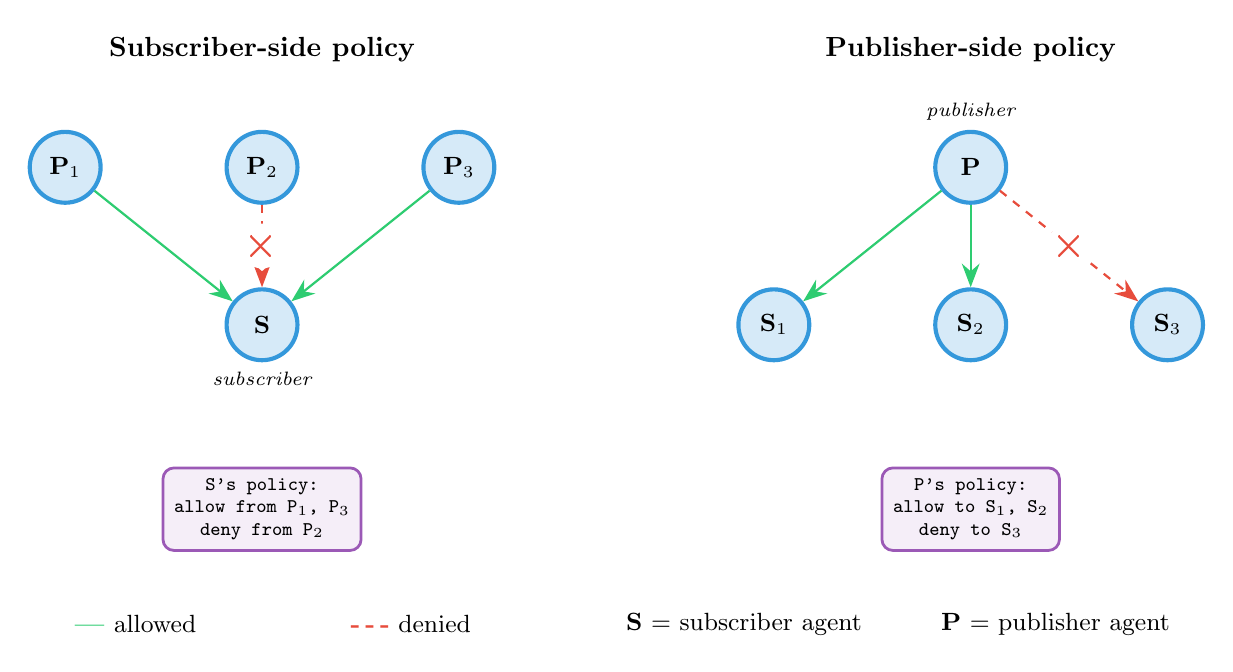
\begin{tikzpicture}[
        agentnode/.style={circle, draw=agent, fill=agent!20, line
        width=1.5pt, minimum size=0.9cm, font=\bfseries\small},
        allowed/.style={-{Stealth[length=3mm]}, thick, admitted},
        blocked/.style={-{Stealth[length=3mm]}, thick, denied, dashed},
        policybox/.style={rectangle, rounded corners, draw=central,
          fill=central!10, line width=1pt, inner sep=4pt,
        font=\scriptsize\ttfamily},
        crossmark/.style={font=\Large\bfseries, text=denied, inner
        sep=0pt, fill=white, circle},
      ]
      % Left scenario: subscriber filters its inputs
      \node[font=\normalsize\bfseries] at (-4.5, 5) {Subscriber-side policy};

      \node[agentnode] (pub1) at (-7, 3.5) {P$_1$};
      \node[agentnode] (pub2) at (-4.5, 3.5) {P$_2$};
      \node[agentnode] (pub3) at (-2, 3.5) {P$_3$};

      \node[agentnode] (subA) at (-4.5, 1.5) {S};
      \node[font=\scriptsize\itshape, anchor=north] at (subA.south)
      {subscriber};

      \draw[allowed] (pub1) -- (subA);
      \draw[blocked] (pub2) -- (subA);
      \node[crossmark] at ($(pub2)!0.5!(subA)$) {\texttimes};
      \draw[allowed] (pub3) -- (subA);

      \node[policybox, anchor=north, align=center] at (-4.5, -0.3)
      {S's policy:\\allow from P$_1$, P$_3$\\deny from P$_2$};

      % Right scenario: publisher restricts subscribers
      \node[font=\normalsize\bfseries] at (4.5, 5) {Publisher-side policy};

      \node[agentnode] (pubB) at (4.5, 3.5) {P};
      \node[font=\scriptsize\itshape, anchor=south] at (pubB.north) {publisher};

      \node[agentnode] (sub1) at (2, 1.5) {S$_1$};
      \node[agentnode] (sub2) at (4.5, 1.5) {S$_2$};
      \node[agentnode] (sub3) at (7, 1.5) {S$_3$};

      \draw[allowed] (pubB) -- (sub1);
      \draw[allowed] (pubB) -- (sub2);
      \draw[blocked] (pubB) -- (sub3);
      \node[crossmark] at ($(pubB)!0.5!(sub3)$) {\texttimes};

      \node[policybox, anchor=north, align=center] at (4.5, -0.3)
      {P's policy:\\allow to S$_1$, S$_2$\\deny to S$_3$};

      % Legend
      \node[font=\small, anchor=west] at (-7, -2.3)
      {\textcolor{admitted}{\textbf{---}}\,\,allowed};
      \node[font=\small, anchor=west] at (-3.5, -2.3)
      {\textcolor{denied}{\textbf{-\,-\,-}}\,\,denied};
      \node[font=\small, anchor=west] at (0, -2.3) {\textbf{S} =
      subscriber agent};
      \node[font=\small, anchor=west] at (4, -2.3) {\textbf{P} =
      publisher agent};
    \end{tikzpicture}
  \end{adjustbox}
  \caption{Per-agent access control. On the left, a subscribing agent
    decides which publishers it will accept messages from. On the
    right, a publishing agent decides which subscribers are allowed to
  receive its messages.}
  \label{fig:peragent-acl}
\end{figure}

This could be implemented in several ways, each with different
trade-offs. Zenoh's existing ACLs can match on certificate common
names, which opens the door to letting each agent carry its own
certificate and writing ACL rules that reference those names
directly~\citep{zenoh-acl,zenoh-firesong}. A simpler path would layer
a policy-check mechanism on top of the message payload, so that
agents handle filtering in application code. A more ambitious path
would extend the central router's administrative API to accept
per-agent policies and translate them into router-level ACL rules.

This idea is clearly preliminary. It depends heavily on how the agent
architecture turns out. If agents end up being dynamic and
short-lived, maintaining per-agent ACL rules could become expensive;
if agents are stable and long-lived, the cost is small. The idea is
recorded here so that when the agent design solidifies, the security
layer can be revisited with this option on the table. It might be
implemented, or it might not.

% ==============================================================
\section{Conclusion}
% ==============================================================

The evaluation confirms that Zenoh is a good fit for the DVerse
platform's communication layer. The pub/sub model is straightforward
to use, and support for multiple topologies gives the flexibility
needed for a decentralized architecture. TLS and mTLS have been
implemented and validated, providing encrypted and mutually
authenticated communication between all nodes~\citep{zenoh-tls}.

The combination of Avahi-based mDNS discovery with TLS-bound
hostnames solves the local discovery problem without reintroducing
centralization and without compromising
security~\citep{rfc6762,avahi}. The resulting architecture, with
central routers per machine, local agents as clients, and an mTLS
mesh between routers, provides a solid foundation for the platform.

The next steps focus on session-level access control, specifically
admittance and topic ACLs, to support multi-session deployments on
the same network~\citep{zenoh-acl}. This moves the platform from
authenticated connectivity to fine-grained authorization.

% ==============================================================
\section*{Glossary}
\addcontentsline{toc}{section}{Glossary}
% ==============================================================

\begin{description}[leftmargin=2.6cm, style=nextline, font=\sffamily\bfseries]
  \item[A record] DNS resource record that maps a hostname to
        an IPv4 address. The mDNS responder publishes A
        records for the \texttt{.local} hostname so that other
        operators can resolve it.
  \item[ACL] Access Control List. In Zenoh, a JSON block in
        the session configuration that defines which subjects
        are allowed or denied on which key expressions and
        message types. Consumed once at session-open time and
        not reloadable at runtime.
  \item[admission] The handshake by which a candidate node
        becomes a member of a DVerse session. The candidate
        publishes a signed \texttt{JoinRequest}; the admin
        replies with an \texttt{AdmissionDecision} that, on
        accept, carries the Megolm session key wrapped in an
        Olm pre-key message.
  \item[AEAD] Authenticated Encryption with Associated Data.
        A symmetric-cipher mode that provides confidentiality
        and integrity in one step. Megolm payload encryption
        is an AEAD construction.
  \item[Avahi] A Linux daemon that implements mDNS/DNS-SD as
        a system-level service. Used in the V2 plan; replaced
        in V3 by the in-process \texttt{mdns-sd} Rust crate.
  \item[browse] The DNS-SD operation that lists service
        instances of a given type (for example
        \texttt{\_dverse.\_tcp.local}) without requiring the
        caller to know any instance names in advance.
  \item[CN] Common Name. The subject field of a TLS
        certificate that DVerse uses as the operator's
        identifier on the fabric.
  \item[CSR] Certificate Signing Request. A blob containing a
        public key and an identity request, sent to a
        certificate authority for signing.
  \item[Curve25519] An elliptic-curve key-exchange primitive
        used by Olm. The framework binds the operator's
        Curve25519 identity key to the TLS certificate through
        a separate ECDSA signature.
  \item[DNS] Domain Name System (RFC 1035). The hierarchical
        name-resolution protocol from which mDNS derives both
        its packet format and its record types.
  \item[DNS-SD] DNS-based Service Discovery (RFC 6763). The
        service-browsing layer that DVerse uses on top of mDNS
        to find peer operators on the local network.
  \item[ECDSA] Elliptic Curve Digital Signature Algorithm.
        The signature scheme used by DVerse leaf certificates
        and by the identity-binding signature.
  \item[Ed25519] An Edwards-curve digital signature algorithm.
        DVerse uses it as the fingerprint half of the
        vodozemac identity, alongside the Curve25519
        encryption key.
  \item[fabric] The set of mutually authenticated Zenoh peers
        connected through the same mTLS-protected mesh.
  \item[\texttt{GroupReceiver}] The Megolm decrypt half. One
        per known peer in the cipher's receivers map.
  \item[JSON5] A superset of JSON that allows comments,
        trailing commas, and unquoted keys. Zenoh's
        configuration files are JSON5.
  \item[JWKS] JSON Web Key Set. The set of public keys that
        Keycloak publishes so that Step-CA can verify the
        signature of a JWT.
  \item[JWT] JSON Web Token. The OIDC \texttt{id\_token} that
        the launcher receives from Keycloak and presents to
        Step-CA during certificate enrolment.
  \item[Keycloak] An open-source identity-and-access
        management product; the OIDC identity provider
        against which Step-CA authenticates.
  \item[link-local] A network scope limited to a single
        physical or logical link, used by mDNS via the
        reserved \texttt{.local} top-level domain.
  \item[LLMNR] Link-Local Multicast Name Resolution
        (RFC 4795). A Microsoft alternative to mDNS that is
        being phased out in favour of mDNS.
  \item[\texttt{mdns-sd}] A pure-Rust mDNS/DNS-SD library. V3
        uses it inside the operator's process instead of
        running Avahi system-side.
  \item[mDNS] Multicast DNS (RFC 6762). Link-local name
        resolution on UDP port 5353; used here to resolve
        operator hostnames without a DNS server.
  \item[Megolm] A group-ratchet cryptographic primitive from
        the Matrix project, used by DVerse to encrypt every
        agent payload under a per-session key.
  \item[mTLS] Mutual Transport Layer Security, in which both
        ends of a TLS connection authenticate with
        certificates.
  \item[multicast] One-to-many network delivery to a group
        identified by a multicast IP address. mDNS uses
        \texttt{224.0.0.251} on IPv4.
  \item[OIDC] OpenID Connect. The identity layer on top of
        OAuth 2.0 that Keycloak implements and that Step-CA
        consumes during enrolment.
  \item[Olm] A one-to-one cryptographic ratchet from the
        Matrix project, used by DVerse to wrap the Megolm
        session key for a specific requester at admission
        time.
  \item[\texttt{ott}] One-time token. Step-CA's name for the
        OIDC \texttt{id\_token} when it is used as a signing
        credential.
  \item[prekey] A short-lived Curve25519 key that the
        admission requester publishes alongside its identity
        key. Used once by the admin's Olm session to
        establish the encrypted channel and discarded
        afterwards.
  \item[provisioner] In Step-CA terminology, a configured
        authentication mechanism (OIDC, JWK, X5C, etc.) used
        to authorise a signing request.
  \item[\texttt{rcgen}] A Rust crate for X.509 certificate
        and CSR generation; used by the launcher to produce
        the local keypair and CSR.
  \item[realm] In Keycloak terminology, an isolated security
        and configuration scope. The DVerse Keycloak deployment
        defines one realm; clients and users live inside it.
  \item[RFC] Request for Comments. The IETF's standards-track
        document series; cited here for mDNS (6762), DNS-SD
        (6763), TLS 1.3 (8446), X.509 (5280), and LLMNR
        (4795).
  \item[SAN] Subject Alternative Name. The extension on an
        X.509 certificate that lists alternative identities
        the certificate is valid for, used here to bind
        \texttt{.local} mDNS names to the cert.
  \item[scope] In OIDC terminology, a request parameter that
        names a set of claims the client requests; DVerse
        uses the \texttt{openid} scope only.
  \item[session] A logical group on the DVerse fabric. Each
        session has its own admin, its own admitted-CN list,
        and its own Megolm session key.
  \item[\texttt{SessionKey}] The Megolm key material
        exchanged during admission and installed by the
        requester as a \texttt{GroupReceiver}.
  \item[Step-CA] An online certificate authority from
        Smallstep; configured with an OIDC provisioner that
        validates JWTs against Keycloak.
  \item[TLS] Transport Layer Security. The DVerse fabric
        runs over TLS 1.3 (RFC 8446) with both ends
        authenticated (\emph{mTLS}).
  \item[TXT record] DNS resource record that carries free-form
        text. DNS-SD uses TXT records to attach key/value
        metadata to a service instance; DVerse publishes the
        operator's CN as a \texttt{cn=} TXT entry.
  \item[vodozemac] A Rust implementation of the Matrix Olm
        and Megolm cryptographic protocols.
  \item[X.509] The ITU-T standard for public-key certificates
        (profiled by RFC 5280) that DVerse uses for leaf
        certificates issued by Step-CA.
  \item[Zenoh] A decentralised pub/sub and query messaging
        protocol from the Eclipse Foundation; the DVerse data
        plane is built on Zenoh sessions.
\end{description}

% ==============================================================
% Bibliography
% ==============================================================
\bibliographystyle{plainnat}
\bibliography{\jobname}

\end{document}
